\section{Annotation Workflows}

\subsection{Adding an annotation}

The following steps must be followed for adding a \KAT annotation:
\begin{figure}[ht]\centering
  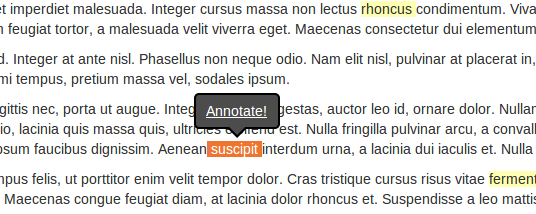
\includegraphics[width=2.5in]{figures/annotate}
  \caption{Selecting the word ``suscipit'' for annotation}\label{fig:kat-annotate}
\end{figure}

\begin{figure}[ht]\centering
 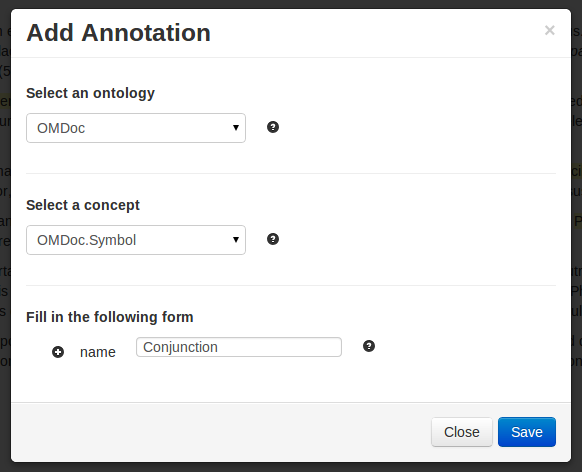
\includegraphics[width=2.5in]{figures/add-symbol}
 \caption{Annotating ``suscipit'' as an OMDoc.Symbol with the name
   ``Conjunction''}\label{fig:kat-symbol}
\end{figure}

\begin{enumerate}
\item The target text of the annotation is highlighted (by simple selection), see Figure~\ref{fig:kat-annotate}
\item The first step triggers an annotation-menu.
\item The annotation-menu is populated with the available annotation types, given by the
  available ontology.
\item The user clicks on the desired annotation concept.
\item A modal box containing the annotation form opens.
\item The annotation form is populated with the fields indicated in the ontology, see Figure~\ref{fig:kat-symbol}
\item After completing the form fields, the user saves the annotation.
\end{enumerate}
This approach ensures 2 things:
\begin{itemize}
\item The navigation flow is never interrupted: adding an annotation is done via pop-up
  and modal boxes and windows, so after completing the steps, the user finds himself in
  the same place in the document.
\item Annotation type checking is implicit: the annotation form is populated with the
  fields indicated in the ontology so the user doesn’t have to check the required types
  himself, see Figure~\ref{fig:kat-definition}
\end{itemize}

\begin{figure}[ht]\centering
 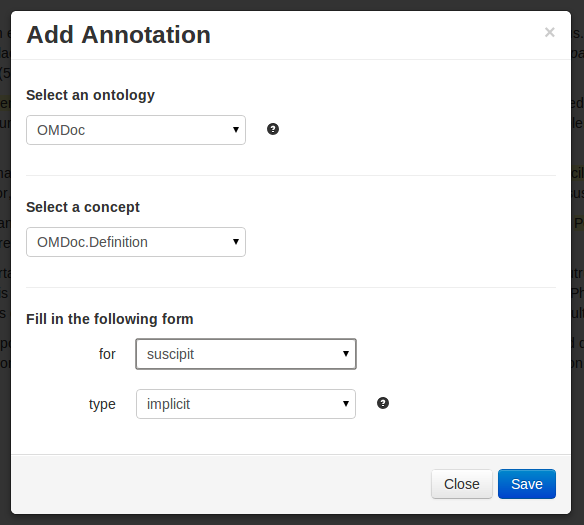
\includegraphics[width=2.5in]{figures/add-definition}
 \caption{Annotating a definition for ``suscipit''. In the ontology, the OMDoc.Definition
   concept is defined to be for annotations of type Symbol. The ``for'' field is
   automatically populated with all the annotations of this type.}\label{fig:kat-definition}
\end{figure}

\subsection{Displaying an annotation}

Annotated text is marked with special CSS style so it becomes easily identifiable.  The
type of the annotation is also displayed above the annotation itself so one can have a
clear overview of the whole document.

At click, a pop-up window containing the annotation display opens.

The annotation display consists of the following elements:
\begin{enumerate}
\item The type of the annotation.
\item The formatted annotation input according to the rules described in the ontology.
\item For the annotations of type reference, an arrow indicated the referenced element.
\end{enumerate}

\begin{figure}[ht]\centering
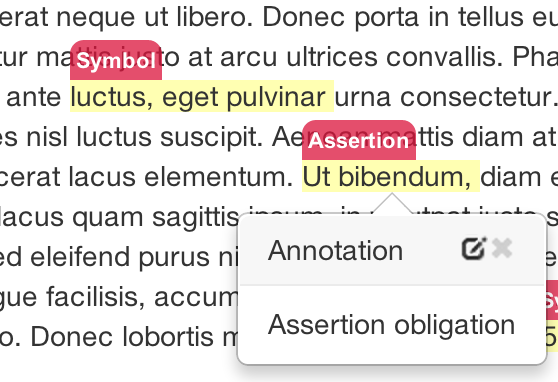
\includegraphics[width=2in]{figures/suscipit}
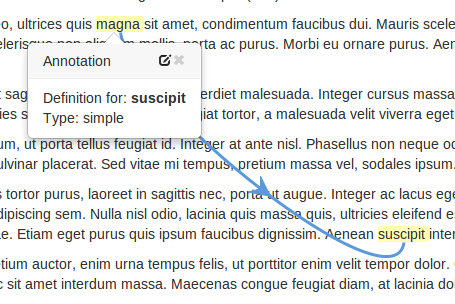
\includegraphics[width=3in]{figures/definition}
\caption{Display for simple text and reference annotations}\label{fig:suscipit-definition}
\end{figure}

\subsection{Reviewing annotation versions}
Reviewing is done in a side-by-side view which allows the user to see two versions of the
same document in order to see discrepancies and correct them; see
Figure~\ref{fig:kat-review}. The viewer allows to toggle view one ontology at a time which
can be toggled individually on each panel by clicking on the.

While reviewing, the left panel (also called the main panel) is the current document with
the local annotations while the right panel (referred to as the mirror panel) is the the
different version of the document being reviewed against.

\KAT is only enabled in the main panel so changes/edits/annotations can still be done
while reviewing, while the mirror panel is read-only. Scrolling the main panel will cause
the mirror panel to automatically follow suite.

\begin{figure}[ht]\centering
 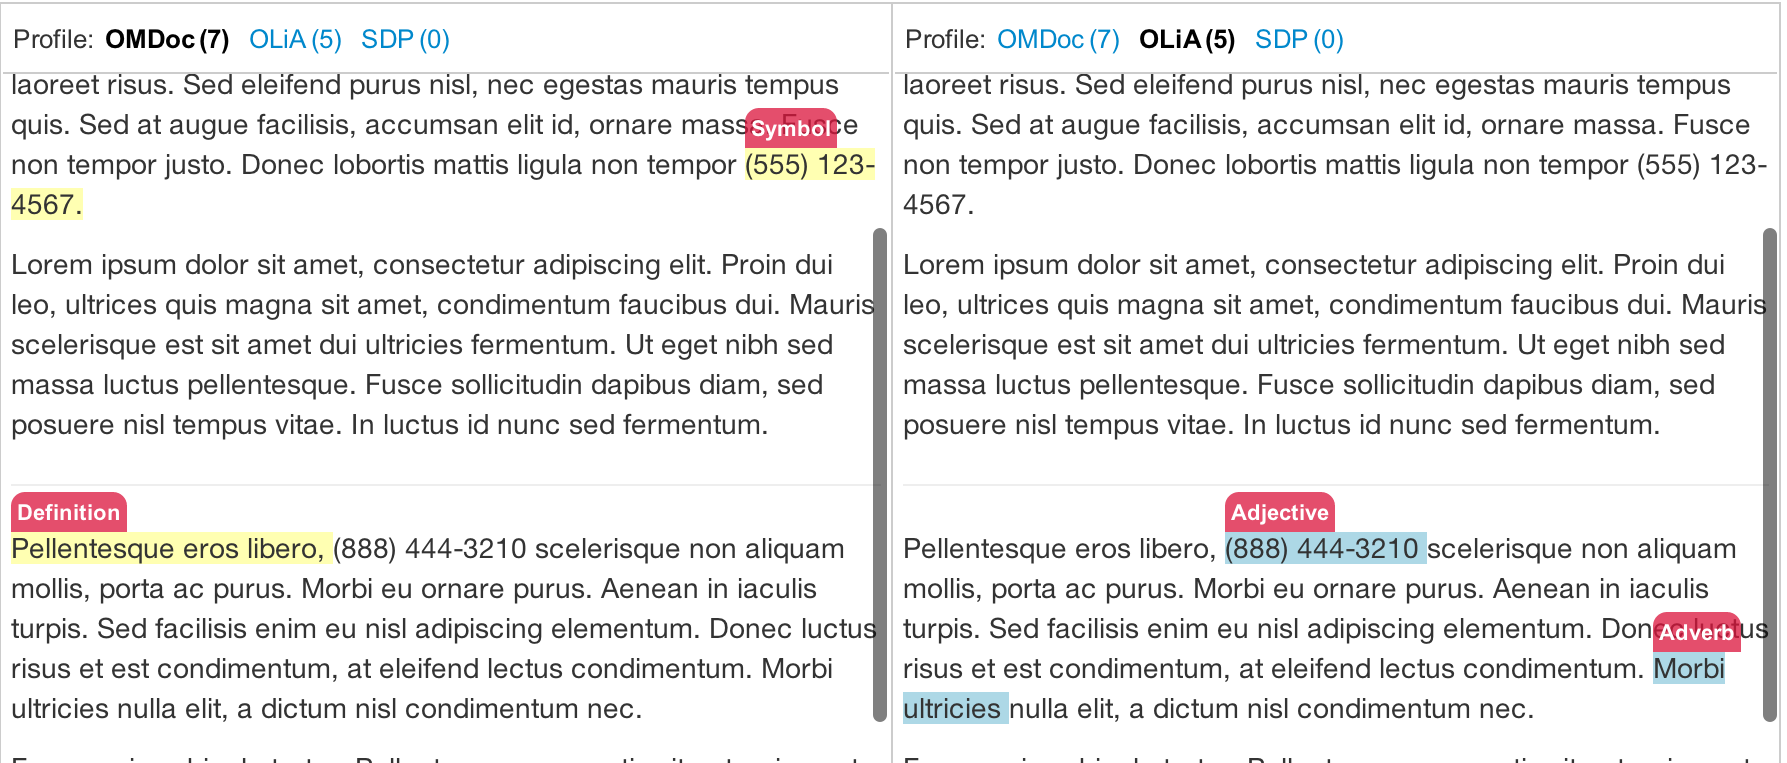
\includegraphics[width=5in]{figures/review}
 \caption{Reviewing two ontologies of the same document side-by-side}\label{fig:kat-review}
\end{figure}

\subsection{Annotating external documents using the browser extension}
A different way of annotating a document which is not part of the corpus is by
using the KAT browser extension. It provides a point-and-click interface which
allows users to easily select the tags they wish to annotate. \\
The following steps must be followed to add an annotation with the KAT browser extension:
\begin{enumerate}
\item Make sure you have the extension installed. You should see the KAT icon near your URL bar.
  Under the icon the extension always displays if the page currently viewed has any annotations or not.
  \begin{figure}[ht]\centering
  
\includegraphics{figures/extension-browser-icon-none}
  \caption{KAT browser icon when viewing a page with no annotations on it}\label{fig:extension-browser-icon-none}
  \end{figure}
\item After loading the page you want to annotate, click the extension icon which will insert a menu in the page. From the menu, choose "Select new tag".
  \begin{figure}[ht]\centering
  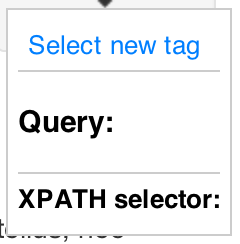
\includegraphics{figures/extension-menu}
  \caption{KAT browser extension menu}\label{fig:extension-menu}
  \end{figure}
\item When moving your mouse around the page, the current tag is always highlighted and its respective DOM and XPATH selectors are displayed in the menu.
  \begin{figure}[ht]\centering
  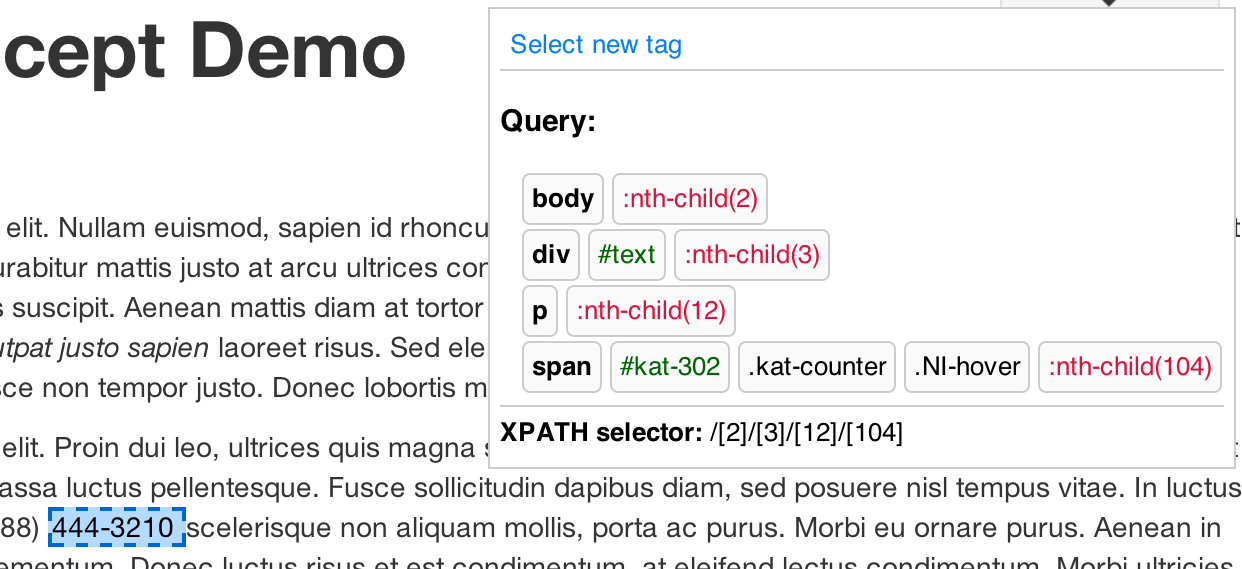
\includegraphics[width=5in]{figures/extension-menu-select}
  \caption{The current tag is always highlighted}\label{fig:extension-menu-select}
  \end{figure}
\item After right clicking on the desired element, the "Annotate" pop-up will appear and the current element will remain selected. Afterwards the work-flow follows the one of adding a normal annotation.
  \begin{figure}[ht]\centering
  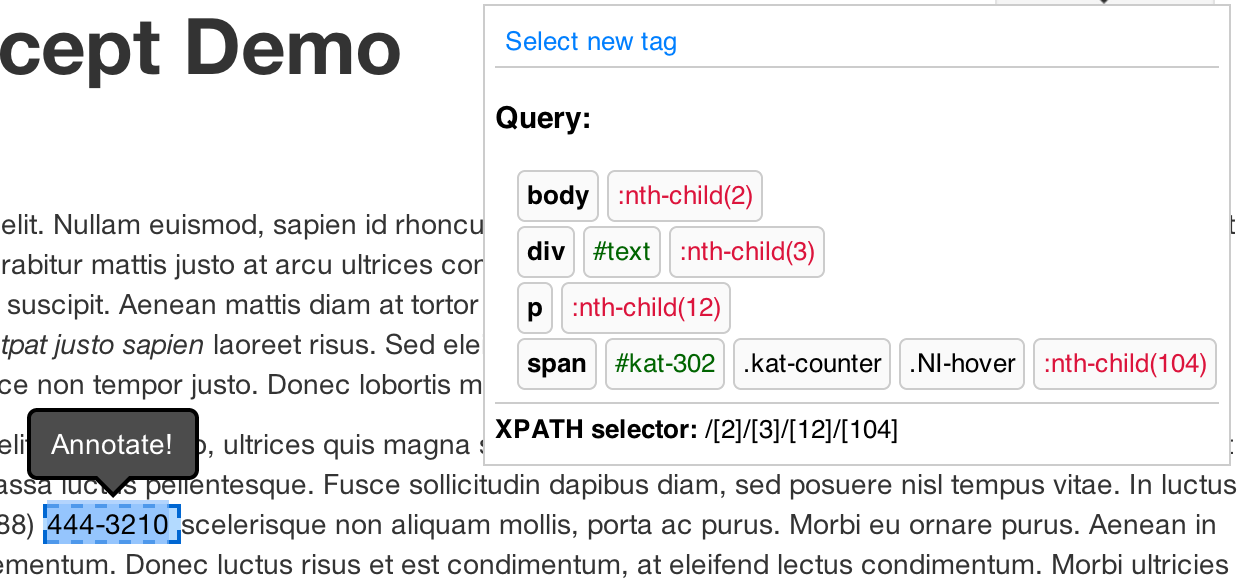
\includegraphics[width=5in]{figures/extension-annotate}
  \caption{Right-clicking on an element causes the "Annotation" pop-up to show}\label{fig:extension-annotate}
  \end{figure}
\item Upon adding an annotation the icon of the extension also changes to reflect the existence of annotations on the current page.
  \begin{figure}[ht]\centering
  
\includegraphics{figures/extension-browser-icon-meta}
  \caption{The icon always changes to reflect the state of the current page}\label{fig:extension-browser-icon-meta}
  \end{figure}
\end{enumerate}

%%% Local Variables:
%%% mode: latex
%%% TeX-master: "kat"
%%% End:
